\section{Auswertung}
\label{sec:Auswertung}
\subsection{Stabilitätsbedingung}
Es wurden die Stabilitätsbedingung des Lasers für zwei
Konfigurationen der Resonatorspiegel überprüft.
Die Stabilitätsbedingung \label{eq:osF} ist für die Konfigurationen in
Tabelle \ref{tab:Konfig} getestet worden.
\begin{table}[H]
    \centering
    \caption{Auflistung der Resonatorspiegelkonfigurationen.}
    \label{tab:Konfig}
    \begin{tabular}{c|c|c|}
        \toprule
        Konfiguration & HR-Spiegel & OC-Spiegel \\
        \midrule
        1 & 1400 mm/flat &1400 mm/flat\\
        2&  flat/flat & 1400 mm/flat\\
        \bottomrule
    \end{tabular}
\end{table}
In den Abbildungen \ref{fig:Konfig1} und \ref{Konfig2} sind die theoretisch bestimmten
Werte aufgeführt, in denen die Stabilitätsbedingung erfüllt ist.
\begin{figure}[H]
  \centering
  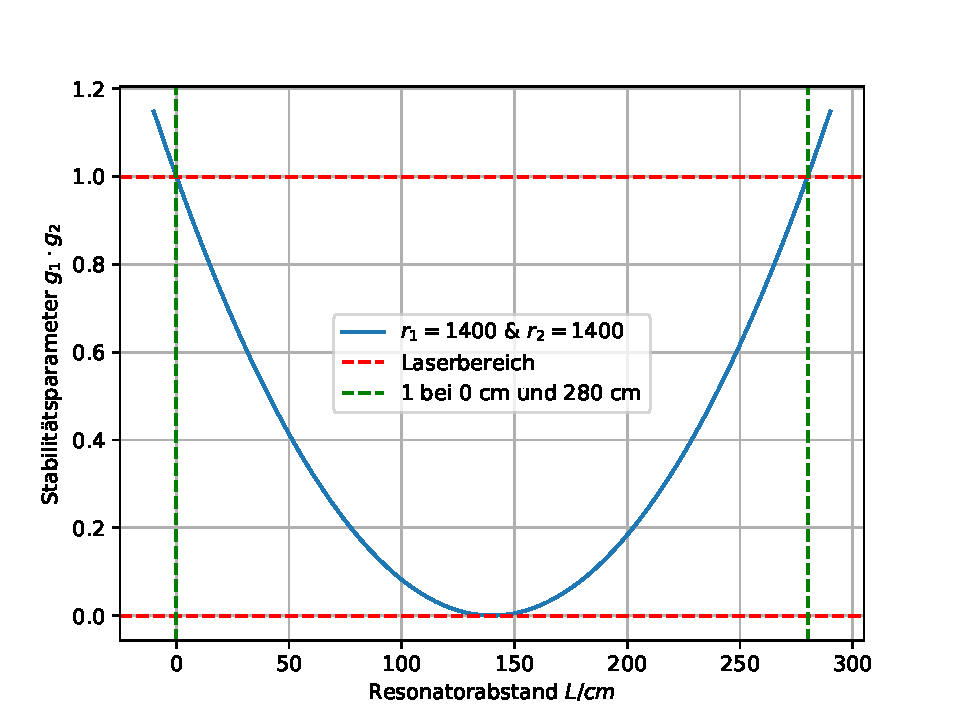
\includegraphics{plots/Vorbereitungsplot2.pdf}
  \caption{Theoretische Berechnung der Stabilitätsbedingung für die erste Konfiguration. Aufgetragen sind
   $g_1 \cdot g_2$ gegen die Resonatorlänge $L$.}
  \label{fig:Konfig1}
\end{figure}

\begin{figure}[H]
  \centering
  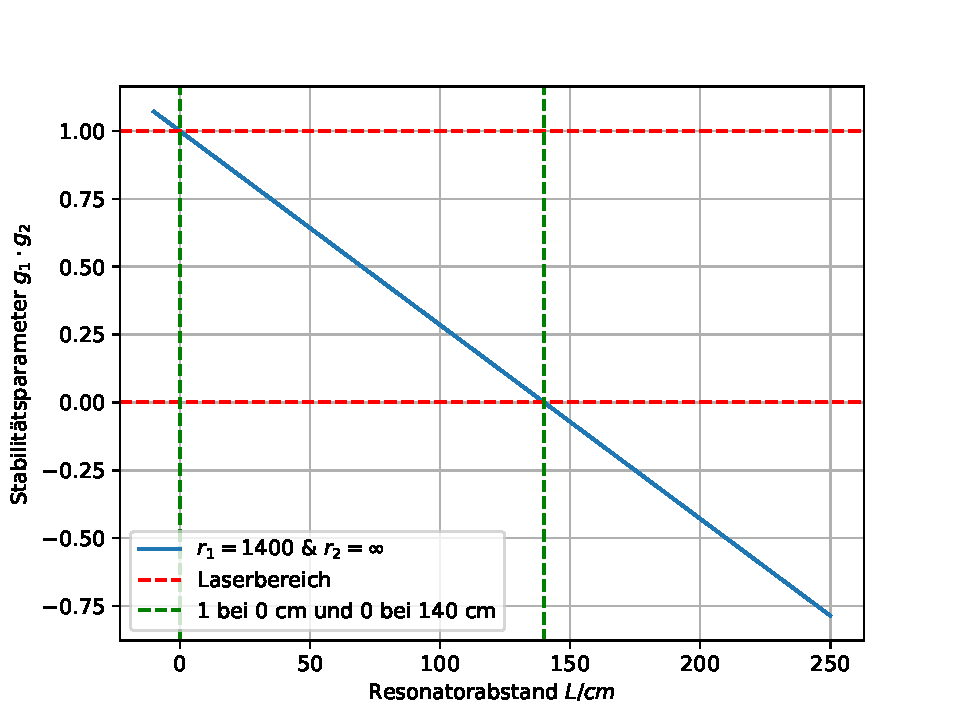
\includegraphics{plots/Vorbereitungsplot1.pdf}
  \caption{Theoretische Berechnung der Stabilitätsbedingung für die zweite Konfiguration. Aufgetragen sind
   $g_1 \cdot g_2$ gegen die Resonatorlänge $L$.}
  \label{fig:Konfig2}
\end{figure}

Im Experiment setzte die Lasertätigkeit bei den in Tabelle \ref{tab:Stabi} aufgeführten
Längen aus.
\begin{table}[H]
    \centering
    \caption{Im Experiment bestimmte maximale Rasonatorlängen für die Konfigurationen 1 und 2.}
    \label{tab:Konfig}
    \begin{tabular}{c|c}
        \toprule
        Konfiguration & $L_{\text{max}}$ in cm  \\
        \midrule
        1 & 191,7\\
        2& 116,7 \\
        \bottomrule
    \end{tabular}
\end{table}

\subsection{Vermessung zweier Moden}
Es werden die Grundmode $\symup{TEM}_{00}$ und die Mode $\symup{TEM}_{01}$ vermessen.
Aus der Formel \ref{eq:Elpq} lässt sich durch das einsetzen der Polynome für die jeweiligen
Parameter und bilden des Betragsquadrates die Intensität der Moden
\begin{align}
  I_{00}{x}&=I\cdot \exp{\left(-\frac{(x-x_{0})^{2}}{\sigma^{2}}\right)}\\
  I_{01}{x}&=I\cdot (x-x_{0})^{2} \exp{\left(-\frac{(x-x_{0})^{2}}{\sigma^{2}}\right)}
  \label{eq:Fit}
\end{align}
bestimmen.
Dabei ist $I$ die maximale Intensität, $x_0$ die Verschiebung der Funktion entlang der
x-Achse und $\sigma$ die Standartabweichung der Verteilung.\\
In den Abbildungen \ref{fig:M00} und \ref{fig:M01} sind die Daten aus Tabelle \ref{tab:DatenModen}
sowie die mittels Ausgleichsrechnung bestimmten Funktionen aus \ref{eq:Fit} dargestellt.
\begin{figure}[H]
  \centering
  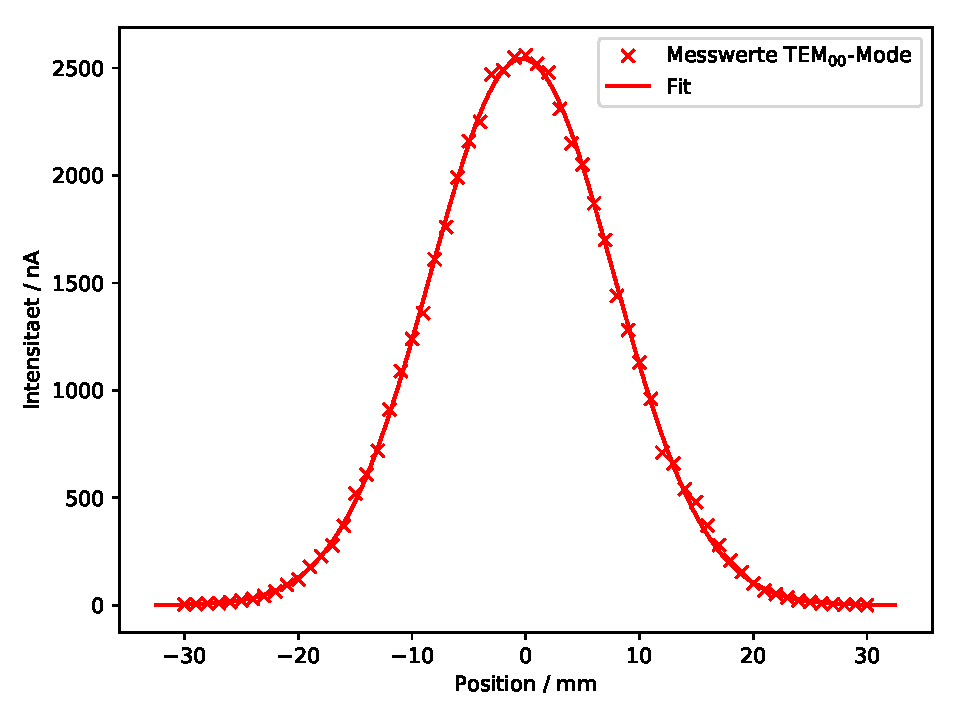
\includegraphics{plots/M00.pdf}
  \caption{Messwerte und Ausgleichskurve der $\text{TEM}_{00}$-Messung.}
  \label{fig:M00}
\end{figure}
Die Parameter für die 00-Mode ergeben sich zu:
\begin{align*}
  I &= (2543 \pm 8)\text{nm}\\
  x_0&=(-0.323 \pm 0.031) \text{mm}\\
  \sigma &= (-16.10 \pm 0.06) \text{mm}^{2}
\end{align*}

\begin{figure}[H]
  \centering
  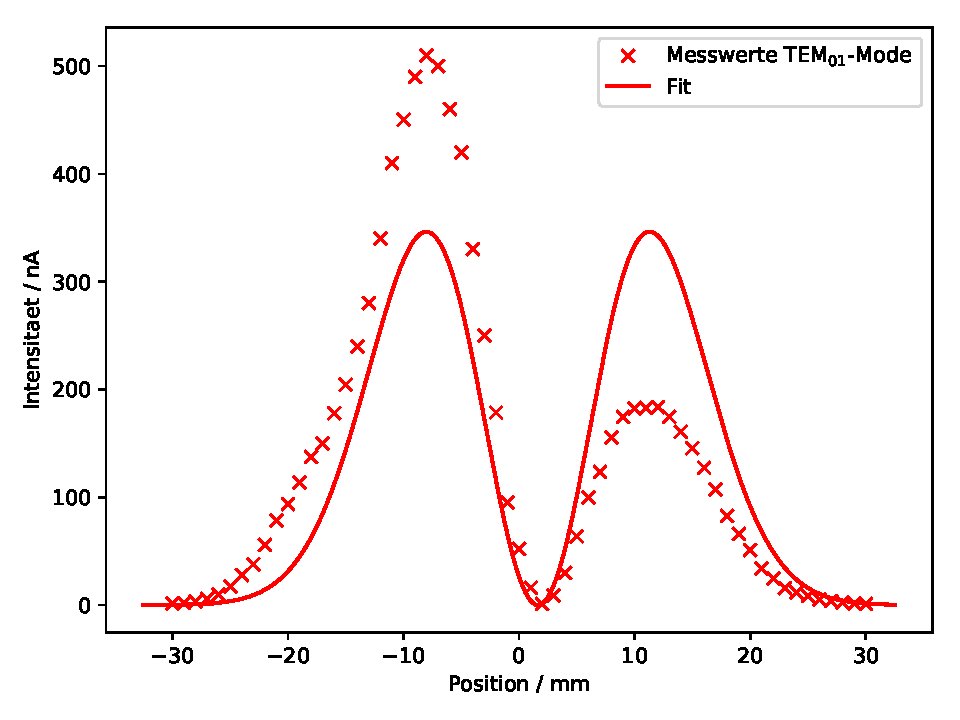
\includegraphics{plots/M01.pdf}
  \caption{Messwerte und Ausgleichskurve der $\text{TEM}_{01}$-Messung.}
  \label{fig:M01}
\end{figure}
Die Parameter für die 01-Mode ergeben sich zu:
\begin{align*}
  I &= (2543 \pm 8)\text{nm}\\
  x_0&=(-0.323 \pm 0.031) \text{mm}\\
  \sigma &= (-16.10 \pm 0.06) \text{mm}^{2}
\end{align*}
